\documentclass{article}

% set font encoding for PDFLaTeX or XeLaTeX
\usepackage{ifxetex}
\ifxetex
  \usepackage{fontspec}
\else
  \usepackage[T1]{fontenc}
  \usepackage[utf8]{inputenc}
  \usepackage{lmodern}
  \usepackage{morefloats}
  \usepackage{wrapfig}
  \usepackage{graphicx}
  \usepackage{float}
\fi

% used in maketitle
\title{Reporte de Actividad 2}
\author{Fátima Brambilla}
\date{07 de Febrero, 2018}

% Enable SageTeX to run SageMath code right inside this LaTeX file.
% documentation: http://mirrors.ctan.org/macros/latex/contrib/sagetex/sagetexpackage.pdf
% \usepackage{sagetex}

\begin{document}
\maketitle

\section{Introducción}
Durante la segunda actividad de "Física Computacional 1", se nos fue introducido el lenguaje de programación \textit{Python}, por medio del "cuaderno de anotaciones" de \textit{Jypiter Notebook}, en el cual trabajamos unos datos obtenidos de la pagina de datos de las Estaciones Automatizadas del Servicio Metereologico Nacional.

\section{Jupyter Notebook}
Jupyter Notebook es un portafolio online, o más bien un servidor que permite a los \textit{clientes} editar y correr documentos. Esta aplicación puede ser ejecutada en el navegador local sin necesidad de estar conectado a la red, o puede ser instalada en un servidor remoto, accediendo a ella a través de una conexión a la web.

\section{Procedimiento}
Después de abrir la terminal en el computador, creamos una carpeta espesífica para la actividad de la semana, y entramos a ella mediante comandos previamente conocidos. Una vez dentro de la carpeta de la actividad, abrimos una nueva terminar, y ejecutamos el comando \textit{jupyter notebook},lo que nos abrio en el navegador una pestaña llamada \textit{home}, la cual se convertiría en nuestra carpeta de trabajo para la actividad.
Lo siguiente fue ejecutar una sesión en \textit{Python 3.0}, lo que nos abrró una ventana más, la cual al principio aparecía sin nombre, de modo que la renombramos \textit{Actividad 2}, ya que ahí trabajaríamos en esta ocasión.
Después, fuimos a la pagina del \textit{Servició Meteorológico Nacional}, para conseguir un archivo de datos. Del mapa nacional que aparecía, se nos pidió seleccionar un Estado y de ahí una de las estaciones, y espesíficar que queríamos los datos con un periodo de 6 minutos. El archivo de texto generado lo descargamos, para posteriormente abrirlo en un editor \textit{emacs}, donde modificamos algunos de los nombres de las columnas de datos.
Una vez hecho esto, se nos pidió visitar un repositorio de Github, donde se encontraba un archivo de Jupyter Notebook, el cual nos serviría de guía y ejemplo para lo que teníamos que hacer.
Dentro del archivo se nos explicaban los pasos que debíamos seguir, así como la manera en que trabajaríamos en Python.
Al completar de modificar un poco el código para que funcionará con nuestros datos, hicimos unas cuantas tablas más por nuestra cuenta.


\section{Observaciones}
La manera de trabajar en Python es bastante diferente a trabajar en Fortran, si bien ambos lenguajes se riguén por un sistema de lógica, la manera de programar en cada uno es diferente, por no mencionar que en Python es más sencillo crear gráficos, algo que hicimos varias veces en este pequeño código.
La primera modificación que hicimos fue en la célula número 13, donde hicimos una gráfico de la variación de la rapidez de los vientos.
En esta gráfica se podía apreciar la variación del viento en metros sobre segundos.
\begin{figure}[H]
    \caption{Variación de la Velocidad del Viento}
    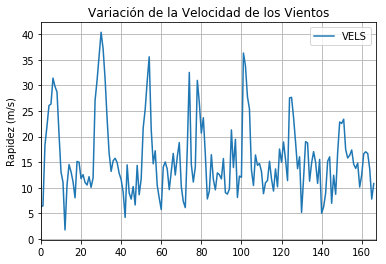
\includegraphics[width=0.5\textwidth]{Variacion VelViento.png}
    \centering
    \label{VeViento}
\end{figure}
La segunda gráfica que generamos era una que comparaba la temperatura con la húmedad relativa, para los datos con los que escogí trabajar no había mucho diferencia, de modo que las lineas se ven bastante juntas en la gráfica.
\begin{figure}[H]
    \caption{Variación de la Temperatura y Húmeda Relativa}
    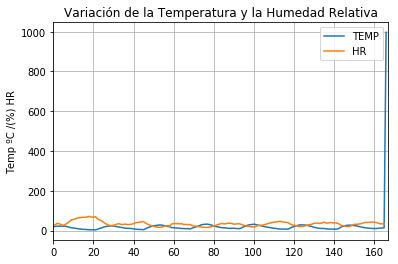
\includegraphics[width=0.5\textwidth]{Variacion Tem-HumRel.png}
    \centering
    \label{TEMHUM}
\end{figure}
La tercera gráfica que trabajamos mostraba la variacón de la temperatura por sí sola. Para mis datos, la variación de la temperatura fue casi nula.
\begin{figure}[H]
    \caption{Variación de la Temperatura}
    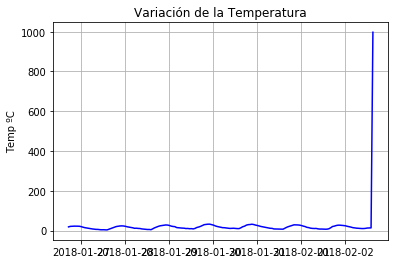
\includegraphics[width=0.5\textwidth]{Variacion Temperatura.png}
    \centering
    \label{TEM}
\end{figure}
Más adelante se nos pidió que hicierámos una gráfica que mostrará la rapidez de los vientos y de las ráfagas como funciones del tiempo.
Hacer esto me llevo unos pocos intentos, porque no estaba segura de que comandos utilizar, pero, al final obtuve el siguiente gráfico:
\begin{figure}[H]
    \caption{Variacion de los Vientos y Ráfagas}
    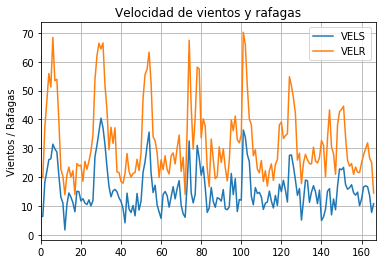
\includegraphics[width=0.5\textwidth]{Vel vientosYrafagas.png}
    \centering
    \label{VelRag}
\end{figure}
Después hicimos una gráfica que mostrara la dirección de los vientos en función del tiempo, en esta gráfica podemos ver como la dirección del viento cambia drásticamente de un día a otro.
\begin{figure}[H]
    \caption{Cambio en la Dirección del Viento}
    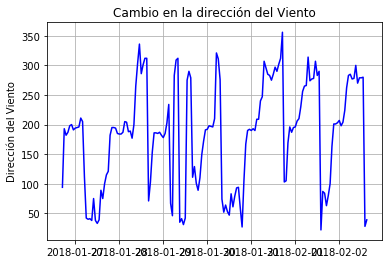
\includegraphics[width=0.5\textwidth]{CambioDirViento.png}
    \centering
    \label{Viento}
\end{figure}

La última gráfica que hicimos comparaba la radiación solar por horas, sin embargo, no encontré la forma de separar los datos para obtener una columna de horas, de modo que mi gráfica muestra la radiación solar por día, de tal manera que no se puede apreciar como cambia durante un solo día.
\begin{figure}[H]
    \caption{Radiación Solar}
    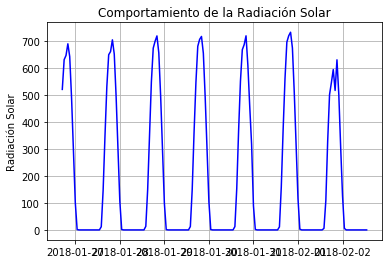
\includegraphics[width=0.5\textwidth]{CompRadiacionSol.png}
    \centering
    \label{RadSol}
\end{figure}
En general, trabajar en Python parece ser más cómodo que en Fortran, pues puedes ver directamente los progresos que llevas sin tener que correr el programa una y otra vez cada que agregas nuevo código.


\section{Bibliografía}

\begin {enumerate}
\item Ingargiola, A. (2015). Jupyter/IPython Notebook Quick Star Guide.
\item Servicio Meteorológico Nacional. (Martes06 de Febrero de 2018). Obtenido de http://smn1.conagua.gob.mx/emas/
\end{enumerate}

\section{Ápendice}
\begin{enumerate}
\item ¿Cuál es tu primera impresión de Jupyter Notebook?
\item ¿Se te dificulto leer código en Python?
\item ¿En base a tu experiencia de programación en Fortran, que te parece el entorno de trabajar en Python?
\item A diferencia de Fortran, ahora se producen las gráficas utilizando las bibliotecas de matplotlib. ¿Cómo fue tu experiencia?
\item En general, ¿Qué te pareció el entorno de trabajo en Python?
\item ¿Qué opinas de la actividad?, ¿Estuvo Compleja?, ¿Qué le falto o que le sobro?,¿Qué modificaste para mejorar?
\item ¿Comentarios adicionales que desees compartir?
\end{enumerate}

Respuestas:
\begin{enumerate}
\item Mi primera impresión fue ladear la cabeza, en un principio no sabía que hacer, o como manejar los comandos de este lenguaje, sin embargo, a medida que iba analizando el código que se nos fue puesto como ejemplo, empecé a notar que trabajar en Python puede ser hasta más sencillo que en Fortran.
\item al principio si, ya que en general estuvimos trabajando únicamente con la creación de gráficas, cosa que rara vez hice en Fortran.
\item Creo que la única diferencia es la retribución que te da el programa, es decir, es más rápido el notar los errores en el código en Python, ya que puedes ejecutar las celdas en las que estas trabajando una por una, y no tienes que correr el programa entero para hacer verificaciones.
\item Fue algo nuevo para mi, ver como las gráficas se crean con tanta facilidad fue sorprendente, ya que en realidad no pude aprender a hacer bien gráficos en Fortran y Gplot.
\item Creo que es un entorno en el cual es sencillo trabajar
\item Pienso que fue una buena actividad para hacer la introducción a Python, y no considero que necesitara algo más o que algo le sobrará.
\item No tengo comentarios adicionales.
\end{enumerate}

\end{document}
